\documentclass[10pt,twocolumn,letterpaper]{article}
\usepackage[margin=0.72in,columnsep=0.26in]{geometry}
\usepackage[T1]{fontenc}
\usepackage{newtxtext}
\usepackage{amsmath,amsthm,graphicx,booktabs,array,multirow,tabularx}
\usepackage[dvipsnames]{xcolor}
\usepackage{tikz}
\usetikzlibrary{arrows.meta,positioning,fit,backgrounds,calc}
\usepackage{microtype,enumitem,fancyhdr}
\usepackage[breaklinks=true,colorlinks=true,citecolor=MidnightBlue,urlcolor=MidnightBlue,linkcolor=MidnightBlue]{hyperref}
\usepackage[numbers,sort&compress]{natbib}
\usepackage{listings}
\lstset{basicstyle=\ttfamily\scriptsize,breaklines=true,frame=single,columns=fullflexible}
\newtheorem{proposition}{Proposition}
\newtheorem{definition}{Definition}
\newcommand{\R}{\mathbb{R}}
\newcommand{\NR}{\textsf{NR}}
\newcommand{\norm}[1]{\left\lVert#1\right\rVert}
\newcommand{\cS}{\mathcal{S}}
\newcommand{\cE}{\mathcal{E}}
\newcommand{\cT}{\mathcal{T}}
\newcommand{\cL}{\mathcal{L}}
\newcommand{\sg}{\operatorname{stopgrad}}
\newcommand{\draftversion}{Revised research draft v2}
\pagestyle{fancy}\fancyhf{}
\fancyhead[L]{\scriptsize EvidenceTrack-GS | Anonymous research draft}
\fancyhead[R]{\scriptsize \draftversion}
\fancyfoot[C]{\thepage}
\setlength{\headheight}{13pt}
\setlength{\emergencystretch}{2em}
\hypersetup{pdftitle={EvidenceTrack-GS: Identity-Controlled Geometry Diagnostics},pdfauthor={Anonymous Authors},pdfsubject={Pre-experiment research draft, not a completed conference submission}}
\title{EvidenceTrack-GS: Identity-Controlled Geometry Diagnostics\\for Diffusion-Assisted Sparse-View Gaussian Splatting}
\author{Anonymous Authors}
\date{}
\begin{document}
\maketitle
\begin{center}\small\textbf{Pre-experiment extended manuscript.}\quad 15 September 2026.\\
Real-scene efficacy is not yet measured. \NR{} means not run, not zero.\\
This editable working layout is not the final official conference template.
\end{center}

\begin{abstract}
Diffusion-enhanced novel views may appear plausible without preserving scene structure. This ambiguity is amplified when a reported gain also includes extra optimization or generic pseudo-view supervision. We develop an identity-controlled protocol around a repaired track-regularized Gaussian baseline and a frozen single-step Difix cache. Track membership, anchors, initialization colors, and confidence use source RGB only, conditional on supplied camera calibration. A shared 10,000-step checkpoint branches into three matched 2,000-step continuations: A1, SelfRender, and B. A1 adds no pseudo-view loss, SelfRender targets frozen A0 renders, and B targets frozen Difix-enhanced A0 renders. Their contrasts separate generic pseudo supervision, the Difix target replacement, and the total B-branch effect. An evaluation-only diagnostic compares source-track queries against projection-only and identity-corrupted controls. We also define failure-aware metrics, camera-coordinate gates, and scene-level paired inference. Historical artifact logs record eleven smoke tests, twenty-three regression tests, and an isolated synthetic recovery result. Those logs predate the current repair and do not validate it. No current-source test, real-scene reconstruction, or real Difix/DINOv2 result is asserted. The protocol is designed to test whether any observed reconstruction change is accompanied by identity-consistent and independent geometric evidence.
\end{abstract}

\section{Introduction}
Three-dimensional Gaussian splatting (3DGS) represents a scene by explicit Gaussian primitives and optimizes them through differentiable rendering~\citep{kerbl2023gaussians}. With only a few source images, many scene explanations remain compatible with the observations. A learned image prior can favor plausible appearance, but plausibility is not a guarantee of correct scene geometry. This distinction is central when a generated image is subsequently used as supervision rather than displayed only as a post-processed rendering.

Frozen diffusion enhancement is an attractive engineering choice because it avoids training a large generator for each reconstruction. Difix3D+ establishes a single-step diffusion route for reconstruction enhancement~\citep{wu2025difix}. Related recent work injects generative cues into feed-forward Gaussian refinement~\citep{chen2026gifsplat}, estimates hallucination-aware reliability for selective distillation~\citep{liu2026had}, or introduces tracker-derived priors into dynamic generation~\citep{sun2025track4dgen}. Consequently, neither ``diffusion plus tracks'' nor ``mask unreliable generated pixels'' is, by itself, a defensible novelty claim.

We instead ask a falsifiable question: \emph{after controlling for source geometry, projection proximity, additional training, and failed matches, do diffusion-enhanced views provide identity-specific geometric utility?} The phrase utility is deliberate. The generator contributes a learned prior, not a new physical sensor observation. A positive answer would motivate a future evidence-driven mechanism; a negative answer would invalidate that motivation before a larger model is built.

The research has three coupled parts. First, a repaired source-track baseline records every anchor's origin and applies geometry loss to current Gaussian centers. Second, three matched continuations separate extra pseudo supervision from replacing self-render targets with Difix targets. Third, an evaluation-only identity diagnostic tests whether source-specific descriptors help beyond searching near a projected location. These parts add no learned adapter, reliability network, or Bayesian posterior fusion. The diagnostic does not feed held-out targets into training.

Our present contributions are a reproducible formulation, an integrity-checked implementation, and experimentally testable attribution criteria. The mathematical statements formalize the limits as well as the advantages of the formulation. They do not turn an unexecuted experiment into an empirical contribution. At this stage, the work should be judged as a detailed pre-experiment research draft rather than a validated state-of-the-art method.

\begin{figure*}[t]
\centering

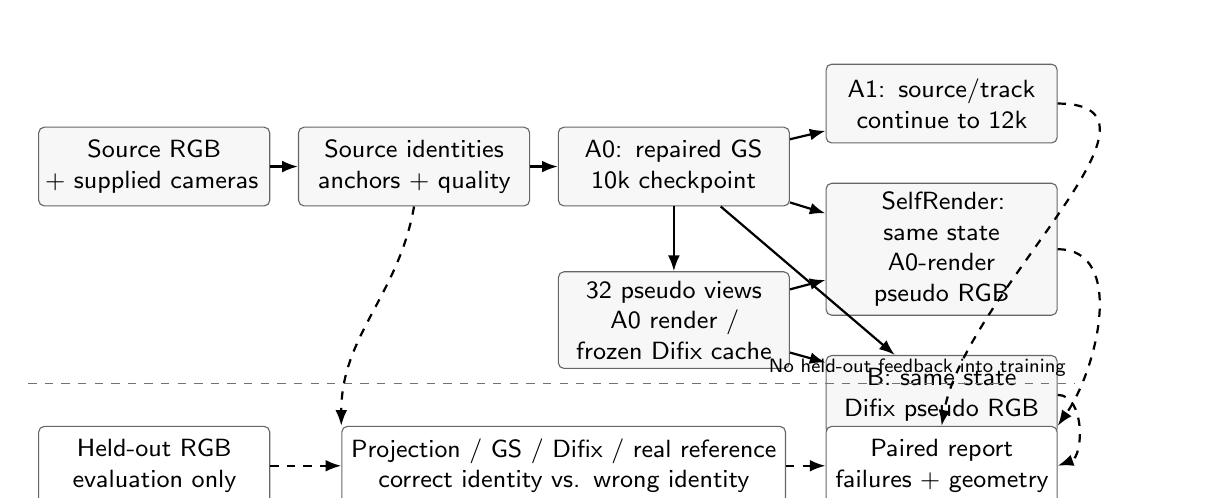
\begin{tikzpicture}[font=\sffamily\small,box/.style={draw=black!60,rounded corners=2pt,align=center,minimum height=10mm,text width=27mm,fill=black!3},arr/.style={-{Latex[length=2mm]},thick}]
\node[box] (src) at (0,1.6) {Source RGB\\+ supplied cameras};
\node[box] (trk) at (3.3,1.6) {Source identities\\anchors + quality};
\node[box] (a0) at (6.6,1.6) {A0: repaired GS\\10k checkpoint};
\node[box] (a1) at (10,2.4) {A1: source/track\\continue to 12k};
\node[box] (self) at (10,.55) {SelfRender: same state\\A0-render pseudo RGB};
\node[box] (b) at (10,-1.3) {B: same state\\Difix pseudo RGB};
\node[box] (cache) at (6.6,-.35) {32 pseudo views\\A0 render / frozen Difix cache};
\draw[arr] (src)--(trk);\draw[arr] (trk)--(a0);\draw[arr] (a0)--(a1);\draw[arr] (a0)--(self);\draw[arr] (a0)--(b);\draw[arr] (a0)--(cache);\draw[arr] (cache)--(self);\draw[arr] (cache)--(b);
\node[box,fill=white] (held) at (0,-2.2) {Held-out RGB\\evaluation only};
\node[box,text width=54mm,fill=white] (diag) at (5.2,-2.2) {Projection / GS / Difix / real reference\\correct identity vs. wrong identity};
\node[box,fill=white] (report) at (10,-2.2) {Paired report\\failures + geometry};
\draw[dashed,black!55] (-1.6,-1.15)--(11.7,-1.15);
\draw[arr,dashed] (held)--(diag);\draw[arr,dashed] (trk.south) to[out=-100,in=90] (diag.north west);
\draw[arr,dashed] (a1.east) to[out=0,in=80] (report.north);
\draw[arr,dashed] (self.east) to[out=0,in=55] (report.north east);
\draw[arr,dashed] (b.east) to[out=0,in=20] (report.east);
\draw[arr,dashed] (diag)--(report);
\node[font=\sffamily\scriptsize,anchor=east] at (11.7,-.95) {No held-out feedback into training};
\end{tikzpicture}

\caption{Implemented scope and evaluation boundary. A fixed A0 checkpoint yields matched A1, SelfRender, and B continuations. SelfRender uses frozen A0 renders; B replaces those targets with frozen Difix outputs. Held-out RGB is used only for final evaluation and diagnostics. Dashed arrows are evaluation-only.}
\label{fig:pipeline}
\end{figure*}

\section{Related Work and Claim Boundaries}
\paragraph{Gaussian reconstruction.} The 3DGS representation and its visibility-aware rasterization are inherited~\citep{kerbl2023gaussians}. We retain per-scene optimization and known camera calibration. The added source-track objective constrains selected Gaussian centers; it does not replace the renderer or solve every unobserved surface. A track-regularized baseline must be compared to the same renderer and initialization without the track term to isolate its effect.

\paragraph{Diffusion-guided reconstruction.} Difix3D+ motivates using a frozen one-step enhancer~\citep{wu2025difix}. We use its official reference-conditioned model rather than claim a new diffusion architecture. GIFSplat uses iterative feed-forward residual updates and diffusion-derived Gaussian cues~\citep{chen2026gifsplat}; our per-scene gradient-based setting differs in inference assumptions and cost. Those differences require separate comparison categories and do not establish superior novelty. HAD estimates hallucination scores and masks unreliable generated pixels using a pretrained feed-forward NVS model~\citep{liu2026had}. The current implementation has no equivalent learned scoring module, and we do not rename a reliability mask as a track-identity contribution.

\paragraph{Tracking and features.} Track4DGen injects tracker-based motion priors into intermediate generative representations and reconstructs dynamic 4D assets~\citep{sun2025track4dgen}. We address static, calibrated scene optimization, but static versus dynamic scope alone is not the key distinction. Our diagnostic uses DINOv2 patch features~\citep{oquab2023dinov2} extracted from RGB images. It does \emph{not} extract internal Difix U-Net features. The RGB feature backend is an implementation control and CPU fixture, not a substitute for pretrained-feature evidence.

\paragraph{What would distinguish the study.} A meaningful outcome would demonstrate, across scenes and seeds, that generated-view utility depends on the correct source-track identity under matched search support, improves geometry beyond projection-only predictions, and survives failure-aware aggregation. The same evidence must also improve reconstruction relative to matched ordinary continuation. Until these conditions are tested, it is inappropriate to claim that the pipeline solves hallucinations or has a stronger generative model than these predecessors.

\section{Setting and Data Provenance}
Let $\cS=\{(I_i,K_i,R_i,t_i)\}_{i=1}^{n}$ be source images with supplied pinhole calibration. A camera maps a world point to $y_i=R_iX+t_i$ and projects it as
\begin{equation}
\pi_i(X)=\begin{bmatrix}f_{xi}y_{ix}/y_{iz}+c_{xi}\\f_{yi}y_{iy}/y_{iz}+c_{yi}\end{bmatrix}.
\end{equation}
The first controlled experiment uses $n=3$; six- and nine-view conditions are preregistered extensions. Images are undistorted before this model is used. An unsupported camera model or missing calibration must be resolved by preprocessing, not silently approximated by an unrelated pinhole model.

Let $\cE$ contain held-out RGB used for evaluation. Source-only in this manuscript means \emph{source-RGB-only geometry construction conditional on supplied calibration}. It does not claim that the camera poses were estimated from three images. Public benchmark poses may have been obtained from a larger image collection; this side information must be disclosed consistently for every method.

A source track $k$ is a set of source image observations $\cT_k=\{(i,u_{ki},c_{ki})\}$, with confidence $c_{ki}$. Source-source matching defines identity before held-out labels are attached. In the strict protocol, full-scene COLMAP point membership and full-scene point coordinates do not define the source track or its initialization. Source point positions, source colors, and quality scores are frozen before any source-to-held-out matching used to build an evaluation table.

Held-out correspondences attached by SIFT matching are \emph{proxy labels}. They are not independent depth ground truth. Requiring agreement from at least two source observations reduces some ambiguity but does not eliminate repeated-texture or occlusion errors. Independent manual correspondence checks and a dataset with genuine geometric reference are therefore required before claiming geometric correctness of novel surfaces.

\paragraph{Audit boundary.} The implementation stores membership provenance, anchor provenance, point-cloud provenance, source names, supplied intrinsics/extrinsics, and source-only confidence. The strict loader verifies the source list against the reconstruction split. Evaluation records may share a file for convenient transport, but training explicitly selects the source portion. We claim a restriction on training contributions, not that the inherited dataset loader never opens a held-out file for evaluation bookkeeping. A server-level deletion/permutation test remains necessary to verify the entire data path, beyond the CPU store fixtures.

\section{Source-Track Geometry}
\subsection{Identity, triangulation, and quality}
The builder extracts SIFT features from the selected source RGB images, uses mutual ratio-tested matching with ratio $0.75$, and filters matches using the given epipolar geometry with a $1.5$-pixel threshold. A union of consistent pairwise matches forms multi-view tracks while rejecting an identity merge that would assign two different features from the same source image to one track. This is an explicit construction of static multi-view correspondences, not a temporal point-tracking model.

For each track observed in at least two sources, linear triangulation supplies an initialization, followed by source-only nonlinear reprojection refinement:
\begin{equation}
\bar X_k=\arg\min_X\sum_{i\in\cT_k}\norm{\pi_i(X)-u_{ki}}_2^2.
\label{eq:triangulation}
\end{equation}
The practical solver is local. Tracks with invalid depth, excessive source reprojection error, or nearly singular local information are rejected. The default maximum mean source residual is $4$ pixels. The source-only initial color is sampled from the track's source observations. No held-out RGB color initializes a Gaussian.

For pixel noise scale $\sigma_p=1$, define $J_{ki}=\partial\pi_i/\partial X$ and local information $H_k=\sum_i J_{ki}^{\mathsf T}J_{ki}/\sigma_p^2$. With $h_k=\operatorname{tr}(H_k)/3$ and relative damping $\eta=10^{-8}$,
\begin{equation}
\Sigma_k=\frac{1}{h_k}\left(\frac{H_k}{h_k}+\eta I\right)^{-1}.
\label{eq:covariance}
\end{equation}
We reject $\lambda_{\min}(H_k)/\lambda_{\max}(H_k)<10^{-10}$. This quantity is a local inverse-information approximation under a pixel-noise model, \emph{not} a calibrated posterior covariance of the full neural reconstruction.

Let $s$ be the median positive pairwise baseline of the source camera centers. Our confidence is
\begin{align}
\nu_k&=\sqrt{\operatorname{tr}(\Sigma_k)}/s,\\
q_k&=\min\!\left(1,\frac{\log(1+m_k)}{\log 7}\right)
\frac{\exp(-e_k/2)}{1+\nu_k},
\label{eq:quality}
\end{align}
where $m_k$ and $e_k$ are source track length and mean source reprojection residual. Both the residual threshold and the exponential are measured in the original source-image pixel convention. Rescaling image resolution is a different operation from changing world units; the quality is not claimed to be invariant to arbitrary image resizing without also rescaling pixel thresholds and noise.

\subsection{The loss must act on current Gaussians}
Let $\mu_j$ be the current center of Gaussian $j$. A track is associated with a nearby Gaussian by an anchor-based nearest-neighbor rule, with a maximum distance of $0.05$ times the source-only camera extent. The association $a(k)$ is fixed while the topology remains unchanged, and recomputed after topology changes. Fixed source-track identity therefore does not imply a permanent Gaussian identifier. Several tracks may associate with one Gaussian; the active count, unique associated count, collision rate, and rejected count are reported.

For the active source observations $\mathcal A$, aggregated across source cameras, use
\begin{equation}
\cL_{\mathrm{trk}}=
\frac{\sum_{(k,i)\in\mathcal A}q_kc_{ki}\,
\rho_\delta(\pi_i(\mu_{a(k)})-u_{ki})}
{\sum_{(k,i)\in\mathcal A}q_kc_{ki}}.
\label{eq:trackloss}
\end{equation}
Here $\rho_\delta(r)$ is a radial Huber penalty on $e=\norm{r}_2$: $e^2/2$ when $e\leq\delta$, and $\delta(e-\delta/2)$ otherwise, with pixel transition $\delta=2$. The threshold is not a world-unit distance. Empty or zero-weight active supervision and non-finite losses are not accepted as successful geometry updates. An explicit smoke test checks that perturbing associated centers produces nonzero, finite gradients with sufficient coverage.

A common implementation error would replace $\mu_{a(k)}$ by the fixed $\bar X_k$ in Eq.~\eqref{eq:trackloss}. That can produce a small reported loss while generating no optimization gradient for the reconstruction. Our loss directly references current Gaussian centers. It nevertheless constrains only associated points; it cannot guarantee accurate density, opacity, occluded surfaces, or appearance elsewhere.

\subsection{Consistent camera coordinates}
A resize by $(s_x,s_y)$ uses pixel-center transport
\begin{equation}
(u',v')=((u+\tfrac12)s_x-\tfrac12,
(v+\tfrac12)s_y-\tfrac12).
\label{eq:pixelresize}
\end{equation}
Focal lengths scale by $s_x,s_y$, and principal points use the same transport. The CUDA renderer's conversion is $u=((x_{\rm ndc}+1)W-1)/2$. The revised projection matrix encodes the actual principal point so that this conversion equals $f_xx/z+c_x$; using only a centered field of view can otherwise misalign the renderer and track loss. The regression suite verifies the algebraic transform. Real CUDA rasterization parity remains a separate server gate.

\section{Frozen Diffusion and Controlled Continuations}
Let $\theta_0$ denote the complete 10,000-step A0 state. From A0, render a source-derived pool of 32 pseudo cameras and choose reference images only from the source set. Define the frozen self-render target $I^0_v=\mathcal R(\theta_0,C_v)$. A fixed reference-conditioned Difix model generates
\begin{equation}
\widetilde I_v=D_W(I^0_v,I_{r(v)};z),
\end{equation}
using the official one-step configuration with timestep $199$, guidance scale $0$, and prompt ``remove degradation''~\citep{wu2025difix}. Model weights and code revisions are recorded. The result is a frozen RGB cache; the generator is not imported into the reconstruction training process. Full-frame output resampling is explicitly recorded so that cached RGB and camera coordinates share one domain.

A1, SelfRender, and B resume from the exact same serialized A0 state. A1 uses source/track training only. SelfRender adds pseudo-view loss toward $I^0_v$, while B replaces that target with $\widetilde I_v$:
\begin{align}
\cL_{A1}&=\cL_{\mathrm{src}}+\lambda_t r_t(t)\cL_{\mathrm{trk}},\\
\cL_{\mathrm{SelfRender}}&=\cL_{A1}+g(t)\lambda_p r_p(t)\cL_{\mathrm{pseudo}}(I^0_v),\\
\cL_B&=\cL_{A1}+g(t)\lambda_p r_p(t)\cL_{\mathrm{pseudo}}(\widetilde I_v),\\
\cL_{\mathrm{pseudo}}(T_v)&=0.8\norm{\mathcal R(\theta,C_v)-T_v}_1
+0.2(1-\mathrm{SSIM}).
\label{eq:lossb}
\end{align}
The source term is the inherited RGB photometric objective. The strict revision disables legacy monocular-depth and pseudo-depth supervision, the optional legacy geometry regularizer, and learned appearance adapters. The repaired track coefficient is $\lambda_t=0.1$. The first experiment uses full precision and freezes topology at 10,000 steps for all continuations. These choices make the branch contrasts auditable; later experiments can relax them symmetrically.

For SelfRender and B, $g(t)=1$ iff $10000<t<12000$ and $t\bmod50=0$; $r_p(t)=\min(1,(t-10000)/500)$ and $\lambda_p=0.1$. Each branch has exactly 39 scheduled pseudo calls cycling through all 32 views. The logged count, ordered camera keys, and unique-view coverage determine whether the protocol was realized. Pseudo calls are interleaved with source updates and are not new physical observations.

\paragraph{Matched state and estimands.} Checkpoints include model tensors, Gaussian-associated auxiliary state, Adam state, random-generator states, and canonical controlled-run provenance. They are written after the declared update, and the final step is not skipped. Legacy incomplete tuples are rejected. A0 embeds the scene, Track and source-image byte inventories, calibrated source cameras, seed, strict geometry settings, and common training protocol. Before its first update, each continuation verifies that object against its current inputs. Each final checkpoint identifies the exact parent A0 path, file hash, and provenance digest; SelfRender and B also identify the strict pseudo manifest, its hash, ordered camera-pool digest, and target kind. The pseudo manifest records the embedded A0 provenance digest used to export its inputs. Source-camera sampling uses a deterministic sequence independent of pseudo sampling. All three continuations must share the A0 hash, real-view sequence, canonical common training-parameter object, exact source-image byte inventory, and calibrated source training-camera payload inventory. Pair-audit v5 requires strict pseudo usage/manifest validation for every pseudo-supervised arm, rehashes each exact final checkpoint, verifies its method role and A0/pseudo lineage, and includes that file in the audited inventory. The held-out v2 and paired v4 evidence records retain the A1/B final-provenance digests through the final association report. SelfRender and B must also share ordered pseudo-camera keys and the realized schedule. SelfRender$-$A1 measures the operational effect of generic pseudo-view supervision toward A0 renders. B$-$SelfRender measures replacing those targets with frozen Difix outputs. B$-$A1 is the total B-branch effect. These interpretations require passed pair audits and do not establish that identity mediates any reconstruction change.

\section{Identity-Controlled Evidence Diagnostic}
\subsection{Queries and matched candidates}
For each source track, bilinearly sample normalized DINOv2 patch features at its source locations and aggregate the source descriptors to obtain $f_k$. Evaluate the same query on three target representations: a GS rendering, its frozen Difix enhancement, and the real held-out image. The real-image branch is a privileged \emph{reference diagnostic}, not a mathematical upper bound: occlusion, textureless regions, and feature-domain behavior may make its score worse than an enhanced image's score.

For target feature map $F_v$ and center $p_{kv}=\pi_v(\bar X_k)$, construct an axis-aligned square candidate window $\Omega_{kv}$ of radius $r=32$ target pixels. With temperature $\tau=0.07$,
\begin{align}
P_{kv}(u)&=\frac{\exp(\langle f_k,F_v(u)\rangle/\tau)}{\sum_{w\in\Omega_{kv}}\exp(\langle f_k,F_v(w)\rangle/\tau)},\\
\widehat u_{kv}&=\sum_{u\in\Omega_{kv}}P_{kv}(u)u.
\label{eq:match}
\end{align}
Entropy and peak similarity are diagnostics, not calibrated correctness probabilities. A local search can return a seemingly good point simply because the window is centered near the true location. A multimodal soft expectation may even lie between two incorrect peaks. Consequently, error alone is insufficient evidence of identity use.

Patch-grid positions correspond to the centers of their image cells, not a linear grid stretched from the first pixel to the last. Source descriptor sampling, target candidate coordinates, and resized evaluation labels obey Eq.~\eqref{eq:pixelresize}. Actual image size, feature size, and effective stride are exported for every target. DINOv2 resolution is therefore not conflated with a three-pixel matching guarantee.

\subsection{Controls and estimands}
The projection-only prediction is $p_{kv}$. The correct-query branch is compared with shuffled source identity, a nearby appearance-similar wrong identity, and a random-query control using the same candidate support. When no distinct hard negative is available, the hard-negative comparison is missing by design; falling back to the same query must not be counted as a successful identity test. The implementation already exports this validity flag. The first figure controls are depicted in Fig.~\ref{fig:null}.

The geometry-relative gain is $e(p_{kv},u^*)-e(\widehat u_{kv},u^*)$; the enhancement gain is the paired error difference between GS-target matching and Difix-target matching. Identity margin compares a wrong-identity query to the correct query under identical target content and candidate support. These are different quantities. A method may improve texture and matching while still fail to outperform the projection-only baseline. A positive identity margin is necessary for an identity-use argument, but is not sufficient proof of correct scene geometry.

Shifted-window tests move the search center by 4, 8, or 16 pixels. The existing GT-inside-window filtering is explicitly labeled \emph{secondary oracle-conditioned analysis}. It must be accompanied by eligibility counts and an unfiltered robustness evaluation before any practical recovery claim is made. Selecting only the successful or easiest windows is not a legitimate main result.

\begin{figure}[t]
\centering
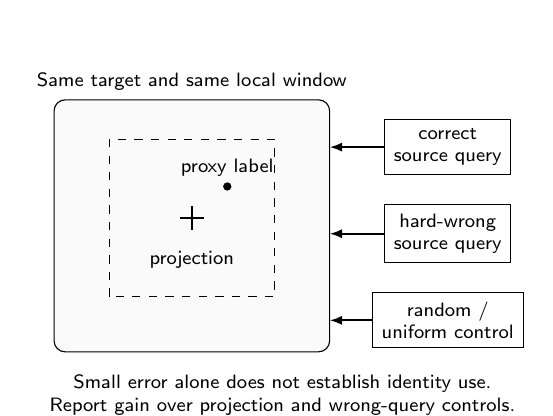
\begin{tikzpicture}[font=\sffamily\scriptsize,arr/.style={-{Latex[length=1.6mm]},thick}]
\draw[rounded corners,fill=black!2] (0,0) rectangle (3.5,3.2);
\draw[dashed] (.7,.7) rectangle (2.8,2.7);
\draw[thick] (1.75,1.55)--(1.75,1.85);\draw[thick] (1.6,1.7)--(1.9,1.7);
\fill (2.2,2.1) circle(1.5pt);\node[above] at (2.2,2.1) {proxy label};
\node[below] at (1.75,1.4) {projection};
\node[above] at (1.75,3.2) {Same target and same local window};
\node[draw,align=center] (correct) at (5,2.6) {correct\\source query};
\node[draw,align=center] (wrong) at (5,1.5) {hard-wrong\\source query};
\node[draw,align=center] (random) at (5,.4) {random /\\uniform control};
\draw[arr] (correct.west)--(3.5,2.6);\draw[arr] (wrong.west)--(3.5,1.5);\draw[arr] (random.west)--(3.5,.4);
\node[align=center] at (2.9,-.55) {Small error alone does not establish identity use.\\Report gain over projection and wrong-query controls.};
\end{tikzpicture}

\caption{A diagnostic can succeed without using identity: a uniform or weak matcher tends toward the local-window center. Correct, hard-wrong, and random queries must share the same candidate set; projection-only remains a required control. This is a schematic, not a measured experiment.}
\label{fig:null}
\end{figure}

\subsection{Failure-aware evaluation}
A prediction is evaluated on a preregistered eligible observation set. PCK at thresholds $3,5,8,16$ pixels counts a missing/non-finite prediction as failure in the denominator. Conditional mean error over successful predictions is reported only alongside coverage, never alone as the principal ranking.

For a complete paired set, define capped error $\ell_v=\min(e_v,d_v)$ for finite predictions and $\ell_v=d_v$ for failures, where $d_v=\sqrt{W_v^2+H_v^2}$ is the common target-image diagonal. This cap makes the failure policy explicit and shared between methods; it is not a learned loss. Also report uncapped successful-match errors and PCK so that the arbitrary severity of the cap is visible. Tracks are averaged within target images and images within scenes. Reconstruction seeds are averaged within scenes before a paired scene bootstrap. Thousands of correlated tracks do not become thousands of independent experimental samples.

\section{Theoretical Analysis and Its Limits}
\subsection{Conditional source-only independence}
\begin{proposition}[No held-out training contribution]
Suppose track membership, anchors, qualities, initial Gaussian state, reference selection, and pseudo cameras are functions only of source RGB $S$, supplied calibration $C$, and fixed random state $Z$. Suppose the diffusion weights $W$ are fixed and no selection or update consults held-out RGB $E$. Then every training iterate is a function $\theta_t=F_t(S,C,W,Z)$, and changing $E$ while holding these inputs fixed cannot change the mathematical training trajectory.
\end{proposition}
\begin{proof}
Initialization satisfies the stated dependence. The frozen cache is a function of the same variables. If $\theta_t$ satisfies the property, the next source sample, pseudo sample, and objective are functions of those variables and $\theta_t$. The optimizer state and update therefore preserve the dependence by induction. Evaluation can read $E$ without violating the conclusion only if its outputs do not alter training, checkpoint selection, thresholds, or stopping.
\end{proof}
This is a structural property, not an assertion that every inherited code path has been dynamically verified. It also does not eliminate information present in externally estimated poses or pretraining data. The artifact includes CPU source-store mutation tests and schedules a full server deletion/permutation test.

\subsection{Scale-equivariant local confidence}
\begin{proposition}[Similarity equivariance]
Under a coordinate change $X'=aQX+b$, $a>0$, orthogonal $Q$, transform cameras as $R_i'=R_iQ^{\mathsf T}$ and $t_i'=a t_i-R_iQ^{\mathsf T}b$. With unchanged pixel observations and noise model, the ideal projected coordinates are unchanged, $\Sigma_k'=a^2Q\Sigma_kQ^{\mathsf T}$ for Eq.~\eqref{eq:covariance}, and $q_k'=q_k$ in Eq.~\eqref{eq:quality} whenever the local information is nondegenerate.
\end{proposition}
\begin{proof}
$R_i'X'+t_i'=a(R_iX+t_i)$, so perspective division is unchanged. By the chain rule, $J_{ki}'=J_{ki}Q^{\mathsf T}/a$ and $H_k'=QH_kQ^{\mathsf T}/a^2$. The trace normalization satisfies $h_k'=h_k/a^2$ and commutes with orthogonal change of coordinates. Substitution into Eq.~\eqref{eq:covariance} yields the covariance transformation. Pairwise camera baselines scale by $a$; hence $s'=as$ and $\sqrt{\operatorname{tr}\Sigma_k'}/s'=\sqrt{\operatorname{tr}\Sigma_k}/s$. Track length and pixel reprojection residual are unchanged.
\end{proof}
Relative damping matters. An additive fixed world-coordinate floor can break this argument. In finite precision, triangulation stopping rules, positive-depth epsilons, and degeneracy guards limit exact equivariance at extreme scales. The new regression test isolates confidence and covariance at five scales from $10^{-6}$ to $10^{6}$; it does not establish invariance of the entire nonlinear training process.

\subsection{Local observability, not global convergence}
\begin{proposition}[Source-ray observability]
For a point with positive depth, a calibrated perspective camera has a rank-two projection Jacobian whose null direction is the viewing ray. For positive weights, $H=\sum_i w_iJ_i^{\mathsf T}J_i$ is positive definite if the source viewing-ray null spaces intersect only at zero. Locally, in the quadratic part of the robust loss, small point perturbations then incur a positive quadratic penalty.
\end{proposition}
\begin{proof}
For camera coordinates $(x,y,z)$, $z>0$,
\begin{equation}
J=\begin{bmatrix}f_x/z&0&-f_xx/z^2\\0&f_y/z&-f_yy/z^2\end{bmatrix}R.
\label{eq:jacobian}
\end{equation}
The first matrix has rank two with null vector $(x,y,z)$. For any vector $v$, $v^{\mathsf T}Hv=\sum_i w_i\norm{J_iv}^2$. The expression is zero exactly when $v$ belongs to every null space. If the intersection is trivial, $H$ is positive definite. A first-order residual expansion produces the claimed local quadratic behavior. For nonzero residuals, the exact Hessian also contains residual-weighted second derivatives, so the positive-definite information matrix is a local Gauss--Newton statement rather than an unrestricted convexity theorem.
\end{proof}
Nearly parallel rays yield poor conditioning even if the matrix is technically full rank. Incorrect correspondences can produce a confidently wrong point. Densification changes the association map, and the joint radiance-field objective is nonconvex. None of these difficulties is resolved by this proposition. The functional recovery test deliberately optimizes only perturbed associated centers with fixed observations to check the narrow mechanism being claimed.

\subsection{Generated views are not independent measurements}
\begin{proposition}[Conditional generated-view information]
Let $X$ be an unknown scene, and let a generated image be $Y=D_W(S,C,Z)$ where $Z$ is conditionally independent of $X$ given $(S,C,W)$. Then
\begin{equation}
I(X;Y\mid S,C,W)=0.
\end{equation}
\end{proposition}
\begin{proof}
Given $(S,C,W)$, the only remaining randomness in $Y$ is the independent $Z$. Therefore $p(Y\mid X,S,C,W)=p(Y\mid S,C,W)$, which is the conditional independence defining zero conditional mutual information.
\end{proof}
The proposition does not say that a pretrained prior is useless. Conditioning on $W$ acknowledges that it can encode population knowledge; a finite-capacity optimizer or representation can benefit from an alternative prior-informed target. It says only that the synthesized samples should not be interpreted as additional independent camera measurements after conditioning on the available inputs and learned prior.

For a scalar illustration, let all $n$ pseudo observations repeat the same noisy value $y=x+\epsilon$, $\operatorname{Var}(\epsilon)=\sigma^2$. Their mean has variance $\sigma^2$, not $\sigma^2/n$. A naive independent-likelihood product shrinks uncertainty by $n$ despite adding no independent noise realization. This is why the present framework does not claim a Bayesian posterior update from 32 generated views and does not equate 32 cache entries with 32 physical measurements.

\subsection{Why locality requires a null control}
For an exactly symmetric candidate window centered at $p$, a uniform matcher has $\widehat u=p$. It can achieve a small error whenever the supplied projection is already close to the proxy target. This statement holds regardless of whether its descriptor contains correct identity information. Finite patch-grid asymmetry changes the barycenter slightly but not the basic confound. Hard-wrong and random queries test descriptor dependence; a projection-only control tests the geometric prior. Their joint use separates mechanisms that a single accuracy score cannot distinguish.

\section{Preregistered Experiments}
\subsection{Datasets, splits, and roles}
The first dataset is LLFF~\citep{mildenhall2019llff}. The eight planned scenes are fern, flower, fortress, horns, leaves, orchids, room, and trex. In the first phase, fern and room are development scenes for engineering and threshold checks. The other six scenes are untouched confirmatory scenes. With the sorted image ordering fixed in the split file, every eighth image is held out and source images are selected deterministically from the remaining images. The exact image-name files, rather than a vague ``three-view setting,'' are the protocol.

We use seeds 1, 2, and 3 for the matched branches and report each seed, the scene mean, and the paired uncertainty. Once a threshold is altered after looking at development results, the change is recorded; confirmatory scenes must not be used for selecting the change. Results pooled over all eight scenes are descriptive, while confirmatory claims use only the untouched subset. Alternative source selections and six-/nine-view settings are robustness tests, not new independent datasets.

DTU geometry and Mip-NeRF 360~\citep{barron2022mip360} are planned extensions. The proposed DTU scan list is 24, 37, 40, 55, 63, 65, 69, 83, 97, 105, 106, 110, 114, 118, 122; it is a preregistered selection, not an asserted reproduction of another paper's exact protocol. Official masks, world units, point-cloud alignment, and evaluation code revisions must be documented before DTU results are interpreted. Mip-NeRF 360 probes unbounded scenes; the generic COLMAP interface does not automatically guarantee that pseudo-camera generation is valid for every unbounded scene.

\subsection{Primary hypotheses and decision rules}
\textbf{H1, functional geometry.} Source-associated Gaussian-center perturbations should produce finite gradients and measurable recovery under the source-only track objective. The server test perturbs centers by $0.005s$, $0.01s$, and $0.02s$ and checks recovery of both reprojection residual and distance to the frozen source anchor. This verifies the training mechanism, not unseen-surface correctness.

\textbf{H2, actual diffusion utility.} At 12,000 updates, B should outperform SelfRender on preregistered held-out reconstruction metrics without an unacceptable geometry regression. This B$-$SelfRender contrast isolates the operational effect of replacing frozen A0-render targets by frozen Difix targets; B$-$A1 measures only the total frozen-Difix branch effect. It does not by itself distinguish a diffusion-specific mechanism from generic enhancement, which requires the planned non-generative enhancement control. LPIPS is a perceptual metric, not a direct surface measurement. A meaningful Difix-target claim requires a favorable paired confidence interval on the primary B$-$SelfRender image contrast and independent geometry evidence; PSNR and SSIM are supporting outcomes. No threshold is retrofitted to make a negative result pass.

\textbf{H3, reconstruction-facing identity evidence.} On the exact shared paired support, B's final GS renders should have lower failure-aware correct-query error and/or a stronger failure-aware valid local hard-negative identity margin than A1's final GS renders. Failure rates and successful-only conditional margins are reported alongside this primary comparison. Difix-target versus GS-target matching remains secondary appearance evidence and cannot replace this reconstruction-facing comparison or independent geometry evaluation. A visual improvement alone cannot satisfy H3.

\textbf{H4, robustness.} Gains should not disappear under modest source changes, feature stride normalization, search-window controls, repetitive texture, or low-overlap scenes. Real-reference matching is reported as context, not used to select successful tracks for the main score.

The principal analysis is a paired scene bootstrap with 10,000 resamples and fixed seed 20260906. Seed-level differences are averaged within scenes before resampling scenes. With only one scene, the implementation refuses to produce a scene confidence interval. With six confirmatory scenes, uncertainty remains limited; more tracks do not solve small scene sample size.

\subsection{Baselines and ablations}
A0 is the shared 10k checkpoint, A1 the 12k source-only continuation, SelfRender the matched continuation supervised by immutable A0 renders, and B the 12k continuation with frozen Difix pseudo RGB. The preregistered contrasts are SelfRender$-$A1 for generic pseudo-supervision, B$-$SelfRender for the diffusion-target replacement, and B$-$A1 for the total B-branch effect. A separate source-initialized renderer without the track term isolates repaired geometry. A simple non-generative image enhancement control is planned to distinguish generic sharpening from a diffusion-specific mechanism.

Ablations vary track weight $\{0,0.03,0.1,0.3\}$, pseudo weight $\{0,0.03,0.1,0.3\}$, local radius $\{16,32,48\}$ pixels, and temperature $\{0.03,0.07,0.15\}$. Pool size and supervision cadence must be varied jointly or their compute and coverage must be reported; a larger cache with unchanged calls is not an equal-coverage comparison. The first controlled run remains fixed at 32/50. Learned scoring, adapter training, and internal diffusion features are explicitly outside this implementation; corresponding proposals cannot appear as completed ablations.

\subsection{Reporting and compute}
Every completed reconstruction run must report dataset, scene, seed, source-name hash, track-store hash, checkpoint hash, model revisions, target resolution, iteration count, Gaussian count, peak GPU memory, source-training time, diffusion-cache time, diagnostic time, and final metrics. GPU timings require synchronization and a stated measurement boundary. Cache generation is not free because it occurs in a second environment. Compare per-scene optimization methods at matched update/compute budgets, and separately disclose pretrained model/data assumptions for feed-forward methods.

\section{Results Available at Draft Time}
\paragraph{Verification status.} Historical artifacts record an environment with Python 3.13.5, PyTorch 2.10.0+cpu, NumPy 2.3.5, and OpenCV 4.13.0, plus eleven Phase-2.1 smoke checks, twenty-three regression tests, and an isolated synthetic recovery. Those artifacts predate the current repair and are not evidence for this source revision. Per the current repair boundary, no current-source CPU test, bootstrap assembly, CUDA extension, real-scene reconstruction, real Difix run, or DINOv2 diagnostic has been executed. The historical Difix reproducibility smoke used a seeded mock pipeline and never established GPU determinism for the real model.

\begin{table}[t]
\centering\small
\begin{tabular}{lrr}
\toprule
Isolated synthetic point test & Initial & Final\\
\midrule
Mean reprojection error (pixels) & 9.7511 & 0.0276\\
Distance to anchor (world units) & 0.053852 & 0.000226\\
Optimization steps & \multicolumn{2}{c}{100}\\
Camera count / optimized point count & \multicolumn{2}{c}{3 / 1}\\
\bottomrule
\end{tabular}
\caption{Historical synthetic fixture from a prior source snapshot. One perturbed point, exact synthetic source observations, fixed cameras, Adam step size 0.01. This is neither a Gaussian-rasterizer benchmark nor a real-scene reconstruction experiment, and it does not validate the current repair.}
\label{tab:synthetic}
\end{table}

\begin{table}[t]
\centering\small
\begin{tabular}{llcccc}
\toprule
Dataset & Branch & PSNR & SSIM & LPIPS & Geometry\\
\midrule
LLFF & A0/A1/SelfRender/B & \NR & \NR & \NR & \NR\\
DTU & A0/A1/SelfRender/B & \NR & \NR & \NR & \NR\\
Mip360 & A0/A1/SelfRender/B & \NR & \NR & \NR & \NR\\
\bottomrule
\end{tabular}
\caption{Research-result registry, not an efficacy table. \NR{} means no corresponding real-scene experiment has been run in this artifact session. Zero, expected scores, literature scores from another protocol, or mock values must not replace these cells.}
\label{tab:registry}
\end{table}

\paragraph{What is not established.} We have not measured real-scene image quality, independent geometry, DINOv2 identity attribution, real Difix reproducibility, peak GPU memory, or runtime. We have not reproduced HAD, GIFSplat, or Track4DGen. No figure contains a generated rendering presented as an experimental output. The schematic figures visualize information flow and controls only. The experiment registry and result-ingestion tools make these missing measurements explicit and reject non-finite or unmeasured values when computing comparisons.

\section{Limitations, Risks, and Responsible Claims}
Sparse source tracks may cover only textured, repeatedly visible surfaces; their absence in a region is not evidence that the region is geometrically reliable. False correspondences can yield false confidence. Nearest-anchor associations can collide or switch after densification, so a track is not a persistent physical Gaussian identity. The local covariance ignores camera uncertainty, occlusion, nonlinear multi-modality, and density/appearance ambiguity. A source-only protocol conditioned on full-scene poses is stricter than full-track geometry reuse but weaker than estimating every input quantity from three images.

The diffusion model may introduce plausible structures unsupported by source images. Independent geometry remains required even if identity margins improve. Descriptor performance and the geometry of local windows can be biased by texture and resolution. Held-out SIFT proxy labels may prefer easy, source-visible regions; independently annotated or ground-truth geometry evaluation must address this selection. Neither the pseudo-image loss nor the current diagnostic provides a mathematical hallucination detector.

On engineering reproducibility, the delivered source overlay and cumulative patch reconstruct the intended pinned project, but their full CUDA installation and real-scene execution require the server gates. A working CPU fixture is not evidence that every GPU branch has been exercised. Upstream code and model licenses remain applicable; pretrained weights and datasets are not redistributed. The internal research package is not automatically an anonymized submission archive.

\section{Conclusion}
We have turned a broad ``diffusion plus tracks'' idea into a falsifiable, source-provenanced reconstruction protocol and an identity-controlled diagnostic. The theory supports local geometric observability, coordinate-consistent confidence, and careful interpretation of generated supervision. Historical CPU logs predate the current repair and do not validate it; efficacy and novelty remain empirical questions. The next decisive evidence is a matched A1/SelfRender/B continuation together with failure-aware, identity-sensitive held-out diagnostics and independent geometry. Stronger architectural claims should follow those results, not precede them.

\clearpage
\appendix
\section{Detailed Mathematical and Implementation Notes}
\subsection{A practical local-conditioning criterion}
For a track with two almost co-located cameras, the viewing rays can be nearly parallel. The minimum eigenvalue of $H_k$ then becomes small relative to its maximum eigenvalue. Rejecting $\lambda_{\min}/\lambda_{\max}<10^{-10}$ prevents the source-quality formula from accepting a numerically invertible but effectively unconstrained triangulation. This is a numerical guard, not a learned rejection probability. The choice is fixed before confirmatory evaluation. An ablation should report the number of rejected tracks as well as downstream quality, since retaining only easy points can improve conditional statistics without improving full-scene reconstruction.

The local covariance computation normalizes by $h_k$ before adding relative damping. Algebraically, Eq.~\eqref{eq:covariance} equals $(H_k+\eta h_kI)^{-1}$. An absolute damping term $\eta I$ would have a different transformation law after changing world units. Floating-point positivity tests and triangulation routines still have finite-range limitations; the claim is an ideal relative-damped local model with numerical tests in specified ranges.

\subsection{Association updates and collision accounting}
Let $N_a$ be the number of associated tracks and $N_u$ the number of unique selected Gaussian indices. Report collision rate $1-N_u/N_a$ when $N_a>0$. A high rate means the effective number of constrained Gaussian variables is lower than the track count. The first implementation does not perform a Hungarian assignment and does not claim one-to-one identity. The server recovery test selects unique associated Gaussian indices and the highest-quality eligible track per selected Gaussian, avoiding an artificial inflation of independent recovery cases.

Association is piecewise constant to avoid differentiating through nearest-neighbor identity changes. This is a pragmatic optimization choice. It creates discontinuities at reassociation and leaves some Gaussians unconstrained. The fixed-topology A1/SelfRender/B experiment removes topology changes from the continuation confound but does not resolve the underlying correspondence problem.

\subsection{Exact camera-center equivalence}
With $x_{\rm ndc}=2f_xx/(Wz)+(2c_x+1)/W-1$, CUDA pixel conversion gives
\begin{align}
u&=\frac{(x_{\rm ndc}+1)W-1}{2}\\
&=f_xx/z+c_x.
\end{align}
The analogous equation holds vertically. This derivation explains why simply assuming $c_x=W/2$ is not a universal calibration policy. The rasterization kernel additionally uses field of view for footprint computations; the calibrated implementation sets field of view from the same focal length. Distortion must already have been removed because the matrix does not model radial or tangential lens distortion.

\subsection{What a diagnostic success would mean}
Suppose a generated image has better LPIPS and source-track matching, but the projection-only coordinate is even more accurate. Such a result supports appearance enhancement and perhaps descriptor stabilization, not new geometric evidence. Suppose correct and shuffled queries perform equally well. Such a result supports a local-search explanation, not identity preservation. Suppose correct-query error improves only after removing failed or shifted-outside-window tracks. Such a result supports a conditional success story, not robust recovery. These outcomes must be retained in the paper, including negative ones.

Even simultaneous positive reconstruction and identity results do not establish that identity matching caused the reconstruction gain: the present diagnostic is not in the optimization loop. The argument would be an association consistent with the hypothesized mechanism. Establishing mediation or a mechanism-specific intervention would require an additional controlled design, which is deliberately not described as implemented here.

\section{Executable Protocol}
\begin{table*}[t]
\centering\small
\begin{tabularx}{\textwidth}{p{0.13\textwidth}p{0.30\textwidth}X}
\toprule
Stage & Executable entry & Required output / stop condition\\
\midrule
Assemble & \texttt{scripts/bootstrap.sh} & Pinned upstream plus cumulative patch and revision. Stops on an existing destination, failed patch check, or unexpected AST structure.\\
CPU gate & \texttt{scripts/run\_cpu.sh} & Current smoke and regression logs, synthetic recovery JSON, and environment record. Historical 11/23 logs do not validate this revision.\\
Track build & \texttt{run\_stage.sh tracks} & Explicit split files and strict HDF5 with source-source membership provenance; audit must retain enough tracks.\\
GPU geometry & \texttt{run\_stage.sh smoke} & Valid current-Gaussian gradients, source-only initialization, no silent empty geometry loss.\\
A0 & \texttt{run\_stage.sh A0} & Complete v2 checkpoint after step 10000; original incomplete checkpoints are rejected.\\
Recovery & \texttt{run\_stage.sh recover} & Read-only checkpoint perturbation/recovery report; do not save modified Gaussian state.\\
Cache & \texttt{export}, then \texttt{cache} & Exactly 32 cameras; fixed source references, model commit, code commit, image hashes, reproducibility check.\\
Continue & \texttt{A1}, \texttt{SelfRender}, then \texttt{B} & Same initial checkpoint; equal source sequence and update count; pseudo branches log 39 calls / 32 unique views and differ only in immutable target kind.\\
Diagnostic & \texttt{evidence-export-a1/b}, \texttt{evidence-cache-a1/b}, \texttt{identity-manifest}, \texttt{identity-a1/b}, then \texttt{identity-report} & Common paired track CSV, feature metadata, unconditional PCK, failure rate, geometry-relative gain and hard-negative validity.\\
Aggregate & \texttt{tools/aggregate\_results.py} & Per-dataset paired scene inference only; rejects unpaired or unmeasured result cells.\\
\bottomrule
\end{tabularx}
\caption{The first experiment is staged so that a failed integrity check stops interpretation before more expensive experiments. Server execution remains outstanding. Paths are relative to the assembled project unless otherwise noted.}
\end{table*}

\paragraph{Environment separation.} Gaussian reconstruction, frozen Difix cache generation, and DINOv2 diagnostics can be run in separate environments because they exchange images, manifests, checkpoints, and HDF5/CSV records. The CPU package lists bounded broad dependencies for testing; it is not a tested CUDA lockfile. Server installation must build the repository's own rasterizer and modified nearest-neighbor extension. In this pinned repository, the nearest-neighbor extension returns a tuple; replacing its use with an assumption from another upstream revision is unsafe.

\paragraph{Immutable inputs.} Select a model revision before real cache generation and store its hash. DINOv2 uses a local pinned official clone; its pretrained weight files also need hashing because pinning only Python source does not pin a downloaded weight URL. Source images and pretrained checkpoints may be large and are not included in this artifact. The commands accept environment variables for these user-supplied paths and revisions rather than invent an unverified server location or model SHA.

\paragraph{Result ingestion.} Do not type expected scores into the experiment tracker. Each row should point to an immutable metric file, its run log, and the corresponding configuration. A0/A1/SelfRender/B reconstruction metrics are measured on held-out RGB at the same resolution and mask policy. Independent DTU geometry results require the official evaluation convention and a documented mapping from learned Gaussians to the evaluated representation. A generic nearest-point distance is not automatically the official benchmark score.

\section{Preregistered Failure Analysis}
The failure gallery should be selected by a declared rule rather than aesthetic preference: the largest paired regressions, a random fixed-seed sample of all scenes, and representative sparse-track or repetitive-texture cases. Each panel should contain source RGB, held-out RGB, A1, SelfRender, and B renderings, the Difix target when relevant, projected source anchor, correct-query match, hard-wrong match, and the validity mask. A caption must state whether a point is measured ground truth or a proxy correspondence.

For track coverage, plot error against source observation count, triangulation conditioning, normalized uncertainty, baseline, target visibility, and feature stride. These plots can reveal where the prior helps or fails, but they are exploratory unless binning and hypotheses were frozen beforehand. Do not choose a confidence threshold on the test distribution to maximize the final score. Missing hard negatives, missing pseudo files, and out-of-frustum candidates must retain explicit denominators.

\section{Revision and Submission Checklist}
The v2 draft separates the real-reference diagnostic from a bound, distinguishes descriptor identity from geometric improvement, changes main metrics to failure-aware paired reporting, and narrows mathematical claims to their assumptions. It also makes source-only conditioning on supplied poses explicit and rejects incomplete continuation checkpoints. Three simulated reviewer perspectives and point-by-point responses accompany this draft. They are internal analytic reviews by one assistant, not external peer review, and they do not certify acceptance.

Before submission, complete real experiments, disclose failed hypotheses, verify closest contemporary work, move detailed proofs and engineering tables into supplementary material as appropriate, and format the actual manuscript using the official submission-year kit. The inspected CVPR 2026 guidelines require an eight-page main paper excluding references; this extended layout deliberately is not presented as compliant with future 2027 requirements. Remove internal repository identities, machine paths, model-user identifiers, and review working notes from any anonymized submission bundle, while preserving third-party license and attribution obligations in the release process.

\bibliographystyle{plainnat}
\bibliography{references}
\end{document}
